% !TEX root = ./busty_transcription.tex
\section{Derivations for non-bursty promoter models}
\label{sec:non_bursty}

In this section we detail the calculation of mean mRNA levels, fold-changes in
expression, and Fano factors for both thermodynamic and kinetic promoter models
in Figure~\ref{fig1:means_cartoons}. These are the results that were quoted but
not derived in Sections~\ref{section_02_means} and \ref{sec:beyond_means} of the
main text. In each of these models, the natural mathematicization of their
cartoons is either an equilibrium model based on statisticla mechanics, or a
chemical master equation. These derivations will go through the specifics of the
models in Figure~\ref{fig1:means_cartoons}. We point the readers to some other
excellent reviews on the general
frameworks~\cite{Bintu2005a,Sanchez2013,Phillips2015a}.

\subsection{Thremodynamic models of gene regulation}
The first class of models we will explore are the so-called thermodynamic models
of gene regulation~\cite{Ackers1982}. The premise for these models is that we
imagine the steps leading to transcription --binding and unbinding of
transcription factors and of RNAP-- to occur in a timescale much faster than the
downstream processes --open complex formation and RNAP
escape~\cite{Browning2004}. What this allows us to do is to assume that the
steps leading to transcription can be modeled as being in quasi-equilibrium.
This is enormously advantageous since we can use the theoretical tools of 
equilibrium statisticla mechanics to model such process.

This means that we can enlist the possible microstates in which we can find the
promoter in order to calculate their probabilities based on quantities such as
molecular counts and interaction energies. We then assume that the gene
expression level is proportional to the probability of finding the promoter in
the transcriptionally active microstate, i.e.,
\begin{equation}
\text{average rate of transcription} = \sum_i r_i p_i,
\label{eq:rate_transcription_si}
\end{equation}
where $i$ labels the distinct states, $p_i$ is the probability of the ith state,
and $r_i$ is the rate of transcription of that state. As mentioned in the main
text, these models can only deal with the mean gene expression level. This is
because the probability space we consider is that of the state of the repressor,
rather than both the state of the repressor and the mRNA counts. Let's now work
through models 1 and 2 from Figure~\ref{fig1:means_cartoons}(B).

\subsubsection{The Two-State Equilibrium Model}
In this simplest model, depicted as (1) in Figure~\ref{fig1:means_cartoons}(B),
the promoter is idealized as existing in one of two states, either repressor
bound or repressor unbound. The rate of transcription
is assumed to be proportional to the fraction of time spent
in the repressor unbound state.
From the relative statistical weights listed in
Figure~\ref{fig1:means_cartoons}(B), the probability $p_U$ of being in the
unbound state is
\begin{equation}
p_U = \left(1 + \frac{R}{N_{NS}} e^{-\beta\Delta\varepsilon_R}\right)^{-1}.
\end{equation}
The mean rate of transcription is then given by $r p_U$, as assumed by
Eq.~\ref{eq:rate_transcription_si}. The mean number of mRNA is
set by the balance of average mRNA transcription and degradation rates,
so it follows that the mean mRNA level is given by
\begin{equation}
\langle m \rangle = \frac{r}{\gamma}
        \left(1 + \frac{R}{N_{NS}} e^{-\beta\Delta\varepsilon_R}\right)^{-1},
\end{equation}
where $r$ is the transcription rate from the repressor unbound state, $\gamma$
is the mRNA degradation rate, $R$ is repressor copy number, $N_{NS}$ is the
number of nonspecific binding sites in the genome where repressors spend most of
their time when not bound to the operator (binding site), $\beta \equiv 1/k_BT$,
and $\Delta\varepsilon_R$ is the binding energy of a repressor to its operator
site. The derivation of this result can be found in~\cite{Phillips2015a}.

The fold-change is  found as the ratio of mean mRNA with and without repressor
as introduced in Eq.~\ref{eq:fc_def}. Invoking that definition results in
\begin{equation}
\text{fold-change}
= \left(1 + \frac{R}{N_{NS}} e^{-\beta\Delta\varepsilon_R}\right)^{-1},
\end{equation}
which matches the form of the master curve in
Figure~\ref{fig1:means_cartoons}(D) with $\rho=1$ and $\Delta F_R = 
\beta\Delta\varepsilon_r - \log (R / N_{NS})$.

In fact it was noted in~\cite{Chure2019} that this two-state model can be viewed
as the coarse-graining of any equilibrium promoter model in which no
transcriptionally active states have transcription factor bound, or put
differently, when there is no overlap between transcription factor bound states
and transcriptionally active states. We will see this explicitly in the 3-state
equilibrium model below, but perhaps surprising is that an analogous result
carries over even to the nonequilibrium models we consider later.

\subsubsection{The Three-State Equilibrium Model}
Compared to the previous model, here we fine-grain the repressor unbound state
into two separate states: empty, and RNAP bound as shown in (2) in
Figure~\ref{fig1:means_cartoons}(B). This picture was used in~\cite{Garcia2011a}
as we use it here, and in~\cite{Razo-Mejia2018} and~\cite{Chure2019} it was
generalized to incorporate small-molecule inducers that bind the repressor. The
effect of this generalization is, roughly speaking, simply to rescale $R$ from
the total number of repressors to a smaller effective number of available
repressors which are unbound by inducers. We point out that the same
generalization can be incorporated quite easily into any of our models in
Figure~\ref{fig1:means_cartoons} by simply rescaling the repressor copy number
$R$ in the thermodynamic models, or equivalently $k_R^+$ in the kinetic models.

The mean mRNA copy number, as derived in Appendix~\ref{sec:non_bursty}
from a similar enumeration of states and weights as the previous model, is
\begin{equation}
\langle m \rangle = \frac{r}{\gamma}
\frac{\frac{P}{N_{NS}} e^{-\beta\Delta\varepsilon_P}}
        {
        1 + \frac{R}{N_{NS}} e^{-\beta\Delta\varepsilon_R}
        + \frac{P}{N_{NS}} e^{-\beta\Delta\varepsilon_P}
        },
\end{equation}
where the new variables are $\Delta\varepsilon_P$, the difference in RNAP
binding energy to its specific site (the promoter) relative to an average
nonspecific background site, and the RNAP copy number, $P$. The fold-change
again follows immediately as
\begin{align}
\text{fold-change}
&= \frac{\frac{P}{N_{NS}} e^{-\beta\Delta\varepsilon_P}}
        {
        1 + \frac{R}{N_{NS}} e^{-\beta\Delta\varepsilon_R}
        + \frac{P}{N_{NS}} e^{-\beta\Delta\varepsilon_P}
        }
\frac{1 + \frac{P}{N_{NS}} e^{-\beta\Delta\varepsilon_P}}
        {\frac{P}{N_{NS}} e^{-\beta\Delta\varepsilon_P}}
\\
&= \left(
1 + \frac{\frac{R}{N_{NS}} e^{-\beta\Delta\varepsilon_R}}
        {1 + \frac{P}{N_{NS}} e^{-\beta\Delta\varepsilon_P}}
\right)^{-1}
\\
&= (1 + \exp(-\Delta F_R - \log\rho))^{-1},
\end{align}
with $\Delta F_R = \beta\Delta\varepsilon_R - \log(R/N_{NS})$ and $\rho = 1 +
\frac{P}{N_{NS}}\mathrm{e}^{-\beta\Delta\varepsilon_P}$ as shown
in~\fig{fig1:means_cartoons}(B). Thus far, we see that the two thermodynamic
models, despite making different coarse-graining commitments, result in the same
functional form for the fold-change in mean gene expression.  We now explore how
kinetic models fare when faced with computing the same observable.

\mrm{THIS NEEDS TO BE FIXED}

Before jumping into the derivations of the general
computation of the mean mRNA level and the Fano factor we will work through the
derivation of an example master equation. In particular we will focus on model 1
from Figure~\ref{fig1:means_cartoons}(C). The general steps are applicable to
all other chemical master equations in this work.

\subsubsection{The Poisson Promoter Nonequilibrium Model}
For our first kinetic model, we  imitate the states considered in the Two-State
Equilibrium Model and consider the simplest possible picture with only two
states, repressor bound and unbound. This is exactly the model used for the main
results of~\cite{Jones2014}. In this picture, repressor association and
dissociation rates from its operator site, $k_R^+$ and $k_R^-$, respectively,
govern transitions between the two states. When the system is in the unbound
state, transcription initiates at rate $r$, which represents a coarse-graining
of all the downstream processes into a single effective rate. mRNA is degraded
at rate $\gamma$ as already exploited in the previous models.

Let $p_R(m,t)$ denote the joint probability of finding the system in the
repressor bound state $R$ with $m$ mRNA molecules present at time $t$. Similarly
define $p_U(m,t)$ for the repressor unbound state $U$. This model is governed
by coupled master equations giving the time evolution of $p_R(m,t)$ and
$p_U(m,t)$~\cite{Sanchez2008, Sanchez2011, Phillips2019} which we can write as
\begin{align}
\begin{split}
\deriv{t}p_R(m,t) =& 
- \overbrace{k_R^- p_R(m,t)}^{R \rightarrow U}
+ \overbrace{k_R^+ p_U(m,t)}^{U \rightarrow R}
+ \overbrace{(m+1)\gamma p_R(m+1,t)}^{m + 1 \rightarrow m}
- \overbrace{\gamma p_R(m,t)}^{m \rightarrow m - 1}
\\
\deriv{t}p_U(m,t) =&\; 
\overbrace{k_R^- p_R(m,t)}^{R \rightarrow U}
- \overbrace{k_R^+ p_U(m,t)}^{U \rightarrow R}
+ \overbrace{rp_U(m-1,t)}^{m-1 \rightarrow m}
- \overbrace{rp_U(m,t)}^{m \rightarrow m + 1}
\\
&+ \overbrace{(m+1)\gamma p_U(m+1,t)}^{m + 1 \rightarrow m}
- \overbrace{\gamma p_U(m,t)}^{m \rightarrow m - 1},
\label{eq:poisson_promoter_cme}
\end{split}
\end{align}
where each term on the right corresponds to a transition between two states of
the promoter as indicated by the overbrace label. In each equation, the first
two terms describe transitions between promoter states due to repressors
unbinding and binding, respectively. The final two terms describe degradation of
mRNA, decreasing the copy number by one, and the terms with coefficient $r$
describe transcription initiation increasing the mRNA copy number by one.
We direct the reader to Appendix~\ref{sec:cme_from_cartoon} for a careful
treatment showing how the form of this master equation follows from the
corresponding cartoon in Figure~\ref{fig1:means_cartoons}.

We can greatly simplify the notation, which will be especially useful for the
more complicated models yet to come, by re-expressing the master equation in
vector form~\cite{Phillips2012}. The promoter states are collected into a vector
and the rate constants are collected into matrices as
\begin{equation}
\vec{p}(m) = \begin{pmatrix} p_R(m) \\ p_U(m) \end{pmatrix},\
\mathbf{K} = \begin{pmatrix} -k_R^- & k_R^+ \\ k_R^- & -k_R^+ \end{pmatrix},\
\mathbf{R} = \begin{pmatrix} 0 & 0 \\ 0 & r \end{pmatrix},\
\label{eq:2state_cme_matrices}
\end{equation}
so that the master equation may be condensed as
\begin{equation}
\deriv{t}\vec{p}(m,t) =
\left( \mathbf{K} - \mathbf{R} - \gamma m \mathbf{I} \right) \vec{p}(m,t)
                + \mathbf{R} \vec{p}(m-1,t)
                + \gamma (m+1) \mathbf{I} \vec{p}(m+1,t),
\label{eq:2state_rep_cme}
\end{equation}
where $\mathbf{I}$ is the identity matrix. Taking steady state by setting time
derivatives to zero, the mean mRNA can be found to be
\begin{equation}
\langle m \rangle = \frac{r}{\gamma}
        \left(1 + \frac{k_R^+}{k_R^-}\right)^{-1},
\label{eq:mean_m_model1}
\end{equation}
with the algebra details again deferred to Appendix~\ref{sec:non_bursty}. Recall
$k_R^+$ is proportional to the repressor copy number, so in computing
fold-change, absence of repressor corresponds to $k_R^+\rightarrow0$. Therefore
fold-change in this model is simply
\begin{equation}
\text{fold-change} = \left(1 + \frac{k_R^+}{k_R^-}\right)^{-1},
\end{equation}
again matching the master curve of~\fig{fig1:means_cartoons}(D) with $\rho=1$.

\subsubsection{Nonequilibrium Model Two - RNAP Bound and Unbound States}
Our second kinetic model depicted in Figure~\ref{fig1:means_cartoons}(C) mirrors
the second equilibrium model of Figure~\ref{fig1:means_cartoons}(B) by
fine-graining  the repressor unbound state of nonequilibrium model 1, resolving
it into an empty promoter state and an RNAP-bound state. Note in this picture,
in contrast with model 4 below, transcription initiation is accompanied by a
promoter state change, in keeping with the interpretation as RNAP-bound and
empty states: if an RNAP successfully escapes the promoter and proceeds to
elongation of a transcript, clearly it is no longer bound at the promoter.
Therefore another RNAP must bind before another transcript can be initiated.

The master equation governing this model is analogous
to Eqs.~\ref{eq:2state_cme_matrices}-\ref{eq:2state_rep_cme} for model 1 above. The
main subtlety arises since transcription initiation accompanies a promoter state
change. This can be understood by analogy to $\mathbf{K}$. The off-diagonal and
diagonal elements of $\mathbf{K}$ correspond to transitions arriving at or
departing from, respectively, the promoter state of interest. If transcription
initiation is accompanied by promoter state changes, we must have separate
matrices for arriving and departing transcription events since the arriving and
departing transitions have different initial copy numbers of mRNA, unlike for
$\mathbf{K}$ where they are the same (see Appendix~\ref{sec:non_bursty}). The
master equation for this model is
\begin{equation}
\deriv{t}\vec{p}(m,t) =
\left( \mathbf{K} - \mathbf{R_D} - \gamma m \mathbf{I} \right) \vec{p}(m,t)
                + \mathbf{R_A} \vec{p}(m-1,t) +
                \gamma (m+1) \mathbf{I} \vec{p}(m+1,t),
\label{eq:3state_rep_cme}
\end{equation}
with the state vector and promoter transition matrix defined as
\begin{equation}
\vec{p}(m) = \begin{pmatrix} p_R(m) \\ p_E(m) \\ p_P(m) \end{pmatrix},\
\mathbf{K} = \begin{pmatrix} -k_R^- & k_R^+ & 0 \\
                        k_R^- & -k_R^+ -k_P^+ & k_P^- \\
                        0 & k_P^+ & -k_P^- 
                \end{pmatrix},
\label{eq:3state_cme_matrices_pt1}
\end{equation}
and the initiation matrices given by
\begin{equation}
\mathbf{R_A} = \begin{pmatrix}
                0 & 0 & 0 \\ 
                0 & 0 & r \\ 
                0 & 0 & 0
                \end{pmatrix},\
\mathbf{R_D} = \begin{pmatrix}
                0 & 0 & 0 \\ 
                0 & 0 & 0 \\ 
                0 & 0 & r
                \end{pmatrix}.
\label{eq:3state_cme_matrices_pt2}
\end{equation}
The elements of $\vec{p}(m)$ encode the probabilities of having $m$ mRNA present
along with the promoter having repressor bound ($R$), being empty ($E$), or
having RNAP bound ($P$), respectively. $\mathbf{R_A}$ describes probability flux
\textit{arriving} at the state $\vec{p}(m)$ from a state with one fewer mRNA,
namely $\vec{p}(m-1)$, and $\mathbf{R_D}$ describes probability flux
\textit{departing} from the state $\vec{p}(m)$ for a state with one more mRNA,
namely $\vec{p}(m+1)$. $\mathbf{K}$ is closely analogous to model 1.

Mean mRNA at steady state is found analogously to model 1, with the result
\begin{equation}
\langle m\rangle = \frac{r}{\gamma}
        \frac{k_R^- k_P^+}
        {k_R^- k_P^+ + k_R^- (k_P^- + r) + k_R^+ (k_P^- + r)},
\label{eq:model2_meanm}
\end{equation}
and with details again deferred to Appendix~\ref{sec:non_bursty}.
Fold-change is again found from the ratio prescribed by Eq.~\ref{eq:fc_def}, from
which we have
\begin{align}
\text{fold-change}
&=      \frac{k_R^- k_P^+}
        {k_R^- k_P^+ + k_R^- (k_P^- + r) + k_R^+ (k_P^- + r)}
        \frac{k_P^+ + k_P^- + r}{k_P^+}
\\
&=      \left(1 + \frac{k_R^+}{k_R^-}
                \frac{k_P^- + r}{k_P^+ + k_P^- + r}
        \right)^{-1}
\\
&=      \left(1 + \frac{k_R^+}{k_R^-}
        \left(1 + \frac{k_P^+}{k_P^- + r}\right)^{-1}
        \right)^{-1},
\end{align}
which follows the master curve of~\fig{fig1:means_cartoons}(D) with $\rho = 1 +
k_P^+/(k_P^- + r)$ as claimed.

\subsubsection{Nonequilibrium Model Three - Multistep Transcription Initiation
and Escape}
One might reasonably complain that the first two ``nonequilibrium'' models we
have considered are straw men. Their steady states necessarily satisfy detailed
balance which is equivalent to thermodynamic equilibrium. Why is this the case?
At steady state there is by definition no net probability flux in or out of each
promoter state, but since the promoter states form a linear chain, there is only
one way in or out of the repressor bound and RNAP bound states, implying each
edge must actually have a net zero probability flux, which is the definition of
detailed balance (usually phrased as equality of forward and reverse transition
fluxes).

Now we consider model 3 in Figure~\ref{fig1:means_cartoons}(C) which allows the
possibility of true nonequilibrium steady-state fluxes through the promoter
states. We point out that this model was considered previously
in~\cite{Mitarai2015} where a comparison was made with model 1 as used
in~\cite{Jones2014}. The authors of~\cite{Mitarai2015} argued that the
additional complexity is essential to properly account for the noise in the mRNA
distribution. We will weigh in on both models later when we consider observables
beyond fold-change.

The master equation governing this model is identical in form to model 2 above,
namely
\begin{equation}
\deriv{t}\vec{p}(m,t) =
\left( \mathbf{K} - \mathbf{R_D} - \gamma m \mathbf{I} \right) \vec{p}(m,t)
                + \mathbf{R_A} \vec{p}(m-1,t) +
                \gamma (m+1) \mathbf{I} \vec{p}(m+1,t),
\end{equation}
but with a higher-dimensional state space and different matrices. The
state vector and promoter transition matrix are now
\begin{equation}
\vec{p}(m) = \begin{pmatrix} p_R(m) \\ p_E(m) \\
                             p_C(m) \\ p_O(m)\end{pmatrix},\
\mathbf{K} = \begin{pmatrix} -k_R^- & k_R^+ & 0 & 0\\
                        k_R^- & -k_R^+ -k_P^+ & k_P^- & 0 \\
                        0 & k_P^+ & -k_P^- - k_O & 0 \\
                        0 & 0 & k_O & 0
                \end{pmatrix},
\end{equation}
with the four promoter states, in order, being repressor bound ($R$), empty
($E$), RNAP closed complex ($C$), and RNAP open complex ($O$). Besides
increasing dimension by one, the only new feature in $\mathbf{K}$ is the
rate $k_O$, representing the rate of open complex formation from
the closed complex, which we assume for simplicity to be irreversible
in keeping with some~\cite{Mitarai2015} but not all~\cite{DeHaseth1998}
past literature. The initiation matrices are given by
\begin{equation}
\mathbf{R_A} = \begin{pmatrix}
        0 & 0 & 0 & 0 \\ 
        0 & 0 & 0 & r \\ 
        0 & 0 & 0 & 0 \\ 
        0 & 0 & 0 & 0
                \end{pmatrix},\
\mathbf{R_D} = \begin{pmatrix}
        0 & 0 & 0 & 0 \\ 
        0 & 0 & 0 & 0 \\ 
        0 & 0 & 0 & 0 \\ 
        0 & 0 & 0 & r
                \end{pmatrix},
\end{equation}
again closely analogous to nonequilibrium model 2.

The expression for mean mRNA is substantially more complicated now, as worked
out in Appendix~\ref{sec:non_bursty} where we find
\begin{equation}
\langle m\rangle = \frac{r}{\gamma}
        \frac{k_R^- k_P^+ k_O}
        {k_R^- [(k_P^+ (k_O + r) + r(k_P^- + k_O)] + k_R^+ r(k_P^- + k_O)},
\label{eq:model3_mean_m}
\end{equation}
which can be simplified to
\begin{equation}
\langle m\rangle
= \frac{r}{\gamma}
\frac{\frac{k_P^+ k_O}{r(k_O + k_P^-)}}
        {1 + \frac{k_P^+ (k_O + r)}{r(k_O + k_P^-)} + \frac{k_R^+}{k_R^-}}.
\end{equation}
The strategy is to isolate the terms involving the repressor, so that now the
fold-change is seen to be simply
\begin{align}
\text{fold-change}
&= \frac{\frac{k_P^+ k_O}{r(k_O + k_P^-)}}
        {1 + \frac{k_P^+ (k_O + r)}{r(k_O + k_P^-)} + \frac{k_R^+}{k_R^-}}
        \frac{1 + \frac{k_P^+ (k_O + r)}{r(k_O + k_P^-)}}
                {\frac{k_P^+ k_O}{r(k_O + k_P^-)}}
\\
&= \left(
        1 + \frac{k_R^+}{k_R^-}
        \left(1 + \frac{k_P^+ (k_O + r)}{r(k_O + k_P^-)}\right)^{-1}
\right)^{-1},
\end{align}
surprisingly reducing to the master curve of~\fig{fig1:means_cartoons}(D) once
again, with $\rho = 1 + \frac{k_P^+ (k_O + r)}{r(k_O + k_P^-)}$.

This example hints that an arbitrarily fine-grained model of downstream
transcription steps may still be collapsed to the form of the master curve for
the means given in Figure~\ref{fig1:means_cartoons}(D), so long as the repressor
binding is exclusive with transcriptionally active states. We offer this as a
conjecture, and we suspect that a careful argument using the King-Altman diagram
method~\cite{King1956, Hill1966} might furnish a ``proof.'' Our focus here is
not on full generality but rather to survey an assortment of plausible models
for simple repression  that have been proposed in the literature.

\subsubsection{Nonequilibrium Model Four - ``Active'' and ``Inactive'' States}
Model 4 in Figure~\ref{fig1:means_cartoons}(C) is at the core of the theory
in~\cite{Razo-Mejia2020}. At a glance the cartoon for this model may appear very
similar to model 2, and mathematically it is, but the interpretation is rather
different. In model 2, we interpreted the third state literally as an RNAP-bound
promoter and modeled initiation of a transcript as triggering a promoter state
change, making the assumption that an RNAP can only
make one transcript at a time. In contrast, in the present model the promoter
state does \textit{not} change when a transcript is initiated. So we no longer
interpret these states as literally RNAP bound and unbound but instead as
coarse-grained ``active'' and ``inactive'' states, the details of which we leave
unspecified for now. We will comment more on this model below when we discuss
Fano factors of models.

Mathematically this model is very similar to models 1 and 2. Like model 1, the
matrix $R$ describing transcription initiation is diagonal, namely
\begin{equation}
\mathbf{R} = \begin{pmatrix}
                0 & 0 & 0 \\ 
                0 & 0 & 0 \\ 
                0 & 0 & r
        \end{pmatrix}.
\end{equation}
The master equation takes verbatim the same form as it did for model 1,
Eq.~\ref{eq:2state_rep_cme}. Meanwhile the promoter transition
matrix $\mathbf{K}$ is the same as Eq.~\ref{eq:3state_cme_matrices_pt1}
from model 2, although we relabel the
rate constants from $k_P^\pm$ to $k^\pm$ to reiterate that these are not simply
RNAP binding and unbinding rates.

Carrying out the algebra, the mean mRNA can be found to be
\begin{equation}
\langle m\rangle = \frac{r}{\gamma}
\frac{k_R^- k^+}
{k_R^- k^+ + k_R^- k^- + k_R^+ k^-},
\end{equation}
and the fold-change readily follows,
\begin{align}
\text{fold-change}
&=      \frac{k_R^- k^+}{k_R^- k^+ + k_R^- k^- + k_R^+ k^-}
        \frac{k_R^- k^+ + k_R^- k^-}{k_R^- k^+}
\\
&=      \left(1 + \frac{k_R^+}{k_R^-}
                \left(1 + \frac{k^+}{k^-}\right)^{-1}
        \right)^{-1},
\end{align}
from which we see $\rho = 1 + k^+/k^-$ as shown in~\fig{fig1:means_cartoons}(C).

\subsubsection{Nonequilibrium Model Five - Bursty Promoter}
The final model we consider shown in Figure~\ref{fig1:means_cartoons}(C) is an
intuitive analog to model 1, with just two states, repressor bound or unbound,
and transition rates between them of $k_R^+$ and $k_R^-$. In model 1, when in
the unbound state, single mRNA transcripts are produced as a Poisson process
with some characteristic rate $r$. The current model by contrast produces, at
some Poisson rate $k_i$, \textit{bursts} of mRNA transcripts.
The burst sizes are assumed to be geometrically distributed with
a mean burst size $b$, which we will motivate in Section~\ref{sec:beyond_means}
when we derive this model as a certain limiting case of model 4.

From this intuitive picture and by analogy to model 1, then, it should be
plausible that the mean mRNA level is
\begin{equation}
\langle m\rangle = \frac{k_i b}{\gamma}
        \left(1 + \frac{k_R^+}{k_R^-}\right)^{-1},
\end{equation}
which will turn out to be correct from a careful calculation. For now, we simply
note that just like model 1, the fold-change becomes
\begin{equation}
\text{fold-change} = \left(1 + \frac{k_R^+}{k_R^-}\right)^{-1}
\end{equation}
with $\rho=1$ also like model 1.
We will also see later how this model emerges as a natural limit of model 4.
\mrm{ENDS HERE}

\mrm{THIS NEEDS TO BE FIXED}
\subsubsection{Noise in the Two-State Promoter, RNAP Bound or Unbound.}

Our second model of constitutive transcription posits an architecture in which
the promoter is either empty or bound by RNAP ~\cite{Phillips2015a,
Phillips2019}. Here,  as shown in model 2 of Figure~\ref{fig2:constit_cartoons}(A),
transcription initiation results in a state transition from the bound to the
unbound state, reflecting the microscopic reality that an RNAP that has begun to
elongate a transcript is no longer available at the start site to begin another.
As shown in Appendix~\ref{sec:non_bursty}, the Fano factor in this model is
given by
\begin{align}
    \nu = 1 -
        \frac{r\rate{k}{P}{+}}
            {\left(\rate{k}{P}{+} + \rate{k}{P}{-} + r\right)
             \left(\gamma + \rate{k}{P}{+} + \rate{k}{P}{-} + r\right)}.
\label{eq:model2_fano}
\end{align}
The problem with this picture is that the Fano factor is always $<1$. To make
 contact with the experimental reality of $\nu>1$ as shown in
 Figure~\ref{fig2:constit_cartoons}(B), clearly some corrections will be needed.
 While this model adds an appealing element of microscopic reality, we are
 forced to reject it as the additional complexity is unable to capture the
 phenomenology of interest. Obviously the promoter state does in fact proceed
 through cycles of RNAP binding, initiating, and elongating, but it seems that
 the super-Poissonian noise in mRNA copy number we want to model must be
 governed by other features of the system.

\subsubsection{Noise in the Three-State Promoter, Multistep Transcription
Initiation and Escape.} 

How might we remedy the deficits of model 2? It is known~\cite{DeHaseth1998}
that once RNAP initially binds the promoter region, a multitude of distinct
steps occur sequentially before RNAP finally escapes into the elongation phase.
Perhaps adding some of this mechanistic detail as shown in model 3 of
Figure~\ref{fig2:constit_cartoons}(A) might rescue the previous model. The next
simplest refinement of that model could consider open complex formation and
promoter escape as separate steps rather than as a single effective step. In
other words, we construct model 3 by adding a single extra state to model 2, and
we will label the two RNAP-bound states as the closed and open complexes,
despite the true biochemical details certainly being more complex. For example,
earlier work extended this model by adding an additional repressor bound state
and did not explicitly consider the limit with no repressor that we analyze
here~\cite{Mitarai2015}. Again, our goal here is not a complete accounting of
all the relevant biochemical detail; this is an exploratory search for the
important features that a model needs to include to square with the known
experimental reality of constitutive expression.

Unfortunately, as hinted at in earlier work~\cite{Mitarai2015}, this model too
has Fano factor $\nu<1$. We again leave the algebraic details for
Appendix~\ref{sec:non_bursty} and merely state the result that
\begin{align}
\nu = 1 - \frac{r k_P^+ k_O}{\mathcal{Z}}
\frac{k_P^+ + k_P^- + k_O + r + \gamma}
    {\mathcal{Z} + \gamma(k_P^+ + k_P^- + k_O + r) + \gamma^2},
\label{eq:model3_fano}
\end{align}
where we defined $\mathcal{Z} = r(k_O + k_P^-) + k_P^+(k_O + r)$ for notational
tidiness. This is necessarily less than 1 for arbitrary rate constants.

In fact, we suspect \textit{any} model in which transcription proceeds through a
multistep cycle must necessarily have $\nu<1$. The intuitive argument compares
the waiting time distribution to traverse the cycle with the waiting time for a
Poisson promoter (model 1) with the same mean time. The latter is simply an
exponential distribution. The former is a convolution of multiple exponentials,
and intuitively the waiting time distribution for a multistep process
should be more peaked with a smaller fractional width than a single
exponential with the same mean.
A less disperse waiting time distribution means transcription initations are
more uniformly distributed in time relative to a Poisson process. Hence the
distribution of mRNA over a population of cells should be less variable compared
to Poisson, giving $\nu<1$.
(In Appendix~\ref{sec:non_bursty} we present a more precise version
of the intuitive arguments in this paragraph.)
Regardless of the merits of this model in describing the noise properties of
constitutive transcription initiation, it ultimately fails the simplest
quantitative feature of the data, namely that the Fano factor $> 1$ and hence
we must discard this mechanistic picture and search elsewhere.
\mrm{ENDS HERE}

\subsection{Derivation of chemical master equation}
\label{sec:cme_from_cartoon}

\begin{figure}[h!]
\centering
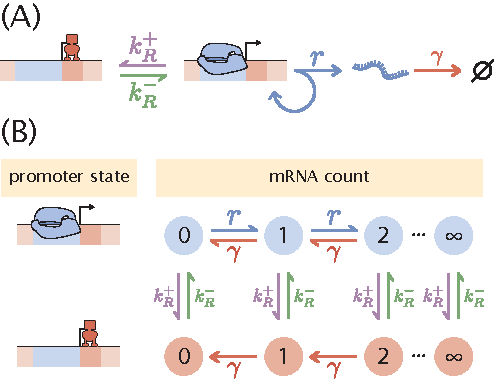
\includegraphics{../../figures/si/figS0X_two_state.pdf}
\caption{
\textbf{Two-state promoter chemical master equation.}
(A) Schematic of the two state promoter simple repression model. Rates $k_R^+$
and $k_R^-$ are the association and dissociation rates of the transcriptional
repressor, respectively, $r$ is the transcription initiation rate, and $\gamma$
is the mRNA degradation rate. (B) Schematic depiction of the mRNA count state
transitions. The model in (A) only allows for jumps in mRNA of size 1. The
production of mRNA can only occur when the promoter is in the transcriptionally
active state.}
\label{fig:two_state}
\end{figure}

The chemical master equation describes the continuous time evolution of a
continuous or discrete probability distribution function. In our specific case
we want to describe the time evolution of the discrete mRNA distribution. What
this means is that we want to compute the probability of having $m$ mRNA
molecules at time $t + \Delta t$, where $\Delta t$ is a sufficiently small time
interval such that only one of the possible reactions take place during that
time interval. For the example that we will work out here in detail we chose the
two-state stochastic simple repression model schematized in
Figure~\ref{fig:two_state}(A). To derive the master equation we will focus more
on the representation shown in Figure~\ref{fig:two_state}(B), where the
transitions between different mRNA counts and promoter states is more explicitly
depicted. Given that the DNA promoter can exist in one of two states --
transcriptionally active state, and with repressor bound -- we will keep track
not only of the mRNA count, but on which state the promoter is. For this we will
keep track of two probability distributions: The probability of having $m$ mRNAs
at time $t$ when the promoter is in the transcriptionally active state $A$,
$p_A(m, t)$, and the equivalent probability but when the promoter is in the
repressor bound state $R$, $p_R(m, t)$.

Since mRNA production can only take place in the transcriptionally active state
we will focus on this function for our derivation. The repressor bound state
will have an equivalent equation without terms involving the production of
mRNAs. We begin by listing the possible state transitions that can occur for a
particular mRNA count with the promoter in the active state. For state changes
in a small time window $\Delta t$ that ``jump into'' state $m$ in the
transcriptionally active state we have
\begin{itemize}
    \item Produce an mRNA, jumping from $m-1$ to $m$.
    \item Degrade an mRNA, jumping from $m+1$ to $m$.
    \item Transition from the repressor bound state $R$ with $m$ mRNAs  to the
    active state $A$ with $m$ mRNAs.
\end{itemize}
Likewise, for state transitions that ``jump out'' of state $m$ in the
transcriptionally inactive state we have
\begin{itemize}
    \item Produce an mRNA, jumping from $m$ to $m+1$.
    \item Degrade an mRNA, jumping from $m$ to $m-1$.
    \item Transition from the active state $A$ with $m$ mRNAs to the repressor
    bound state $R$ with $m$ mRNAs.
\end{itemize}
The mRNA production does not depend on the current number of mRNAs, therefore
these state transitions occur with probability $r\Delta t$. The same is true for
the promoter state transitions; each occurs with probability $k_R^\pm \Delta t$.
As for the mRNA degradation events, these transitions depend on the current
number of mRNA molecules since the more molecules of mRNA there are, the more
will decay during a given time interval. Each molecule has a constant
probability $\gamma \Delta t$ of being degraded, so the total probability for an
mRNA degradation event to occur is computed by multiplying this probability by
the current number of mRNAs.

To see these terms in action let us compute the probability of having $m$ mRNA
at time $t + \Delta t$ in the transcriptionally active state. This takes the 
form
\begin{equation}
\begin{aligned}
p_A(m, t + \Delta t) &= p_A(m, t) \\
&+ \overbrace{(r\Delta t) p_A(m-1, t)}^{m-1 \rightarrow m}
- \overbrace{(r\Delta t) p_A(m, t)}^{m \rightarrow m+1}\\
% \;\;\;\text{(mRNA production)} \\
&+ \overbrace{(m+1)(\gamma \Delta t) p_A(m+1, t)}^{m+1 \rightarrow m}
- \overbrace{m(\gamma \Delta t) p_A(m, t)}^{m \rightarrow m-1}\\
% \;\;\;\text{(mRNA degradation)} \\
&+\overbrace{(k_R^- \Delta t) p_R(m, t)}^{R \rightarrow A}
-\overbrace{(k_R^+ \Delta t) p_A(m, t)}^{A \rightarrow R},
% \;\;\;\text{(promoter state transition)}
\end{aligned}
\end{equation}
where the overbrace indicates the corresponding state transitions. Notice that
the second to last term on the right-hand side is multiplied by $p_R(m, t)$
since the transition from state $R$ to state $A$ depends on the probability of
being in state $R$ to begin with. It is through this term that the dynamics of
the two probability distribution functions ($p_R(m,t)$ and $p_A(m,t)$) are
coupled. An equivalent equation can be written for the probability of having $m$
mRNA at time $t + \Delta t$ while in the repressor bound state, the only
difference being that the mRNA production rates are removed, and the sign for
the promoter state transitions are inverted. This is
\begin{equation}
\begin{aligned}
p_R(m, t + \Delta t) &= p_R(m, t) \\
&+ \overbrace{(m+1)(\gamma \Delta t) p_R(m+1, t)}^{m+1 \rightarrow m}
- \overbrace{m(\gamma \Delta t) p_R(m, t)}^{m \rightarrow m-1}\\
% \;\;\;\text{(mRNA degradation)} \\
&-\overbrace{(k_R^- \Delta t) p_R(m, t)}^{R \rightarrow A}
+\overbrace{(k_R^+ \Delta t) p_A(m, t)}^{A \rightarrow R}.
\end{aligned}
\end{equation}

All we have to do now are simple algebraic steps in order to simplify the 
equations. Let us focus on the transcriptionally active state $A$. First we will
send the term $p_A(m, t)$ to the right-hand side, and then we will divide both
sides of the equation by $\Delta t$. This results in
\begin{equation}
\begin{aligned}
\frac{p_A(m, t + \Delta t) - p_A(m, t)}{\Delta t} &=
r p_A(m-1, t) - r p_A(m, t)\\
&+ (m+1)\gamma p_A(m+1, t)
- m \gamma p_A(m, t)\\
&+k_R^- p_R(m, t)
-k_R^+ p_A(m, t).
\end{aligned}
\end{equation}
Upon taking the limit when $\Delta t \rightarrow 0$ we can transform the 
left-hand side into a derivative, obtaining the chemical master equation
\begin{equation}
\begin{aligned}
\frac{d p_A(m, t)}{dt} &=
r p_A(m-1, t) - r p_A(m, t)\\
&+ (m+1)\gamma p_A(m+1, t)
- m \gamma p_A(m, t)\\
&+k_R^- p_R(m, t)
-k_R^+ p_A(m, t).
\end{aligned}
\end{equation}
Doing equivalent manipulations for the repressor bound state gives an ODE of the
form
\begin{equation}
\begin{aligned}
\frac{d p_R(m, t)}{dt} &=
(m+1)\gamma p_R(m+1, t)
- m \gamma p_R(m, t)\\
&-k_R^- p_R(m, t)
+k_R^+ p_A(m, t).
\end{aligned}
\end{equation}
In the next section we will write these coupled ODEs in a more compact form using
matrix notation.

\subsection{Matrix form of the multi-state chemical master equation}

Having derived an example chemical master equation we now focus on writing a
general matrix form for the kinetic models 1-4 shown in
Figure~\ref{fig1:means_cartoons}(C) in the main text. In each of these four
models, the natural mathematicization of their cartoons is as a chemical master
equation such as Eq.~\ref{eq:2state_rep_cme} for model 1, which for
completeness we reproduce here as
\begin{align}
\begin{split}
\deriv{t}p_R(m,t) =& 
- \overbrace{k_R^- p_R(m,t)}^{R \rightarrow U}
+ \overbrace{k_R^+ p_U(m,t)}^{U \rightarrow R}
+ \overbrace{(m+1)\gamma p_R(m+1,t)}^{m + 1 \rightarrow m}
- \overbrace{\gamma mp_R(m,t)}^{m \rightarrow m - 1}
\\
\deriv{t}p_U(m,t) =&\; 
\overbrace{k_R^- p_R(m,t)}^{R \rightarrow U}
- \overbrace{k_R^+ p_U(m,t)}^{U \rightarrow R}
+ \overbrace{rp_U(m-1,t)}^{m-1 \rightarrow m}
- \overbrace{rp_U(m,t)}^{m \rightarrow m + 1}
\\
&+ \overbrace{(m+1)\gamma p_U(m+1,t)}^{m + 1 \rightarrow m}
- \overbrace{\gamma mp_U(m,t)}^{m \rightarrow m - 1}.
\label{eq:poisson_promoter_cme_appdx}
\end{split}
\end{align}
Here $p_R(m,t)$ and $p_U(m,t)$ are the probabilities of finding the system with
$m$ mRNA molecules at time $t$ either in the repressor bound or unbound states,
respectively. $r$ is the probability per unit time that a transcript will be
initiated when the repressor is unbound, and $\gamma$ is the probability per
unit time for a given mRNA to be degraded. $k_R^-$ is the probability per unit
time that a bound repressor will unbind, while $k_R^+$ is the probability per
unit time that an unbound operator will become bound by a repressor. Assuming
mass action kinetics, $k_R^+$ is proportional to repressor copy number $R$.

Next consider the cartoon for nonequilibrium model 2 in
Figure~\ref{fig1:means_cartoons}(C). Now we must track probabilities $p_R$,
$p_P$, and $p_E$ for the repressor bound, empty, and polymerase bound states,
respectively. By analogy to Eq.~\ref{eq:poisson_promoter_cme_appdx}, the master
equation for model 2 can be written
\begin{align}
\begin{split}
\deriv{t}p_R(m,t) =& 
- \overbrace{k_R^- p_R(m,t)}^{R \rightarrow U}
+ \overbrace{k_R^+ p_E(m,t)}^{U \rightarrow R}
+ \overbrace{(m+1)\gamma p_R(m+1,t)}^{m + 1 \rightarrow m}
- \overbrace{\gamma mp_R(m,t)}^{m \rightarrow m - 1}
\\
\deriv{t}p_E(m,t) =&\; 
  \overbrace{k_R^- p_R(m,t)}^{R \rightarrow U}
- \overbrace{k_R^+ p_E(m,t)}^{U \rightarrow R}
+ \overbrace{(m+1)\gamma p_E(m+1,t)}^{m + 1 \rightarrow m}
- \overbrace{\gamma mp_E(m,t)}^{m \rightarrow m - 1}.
\\
&
+ \overbrace{k_P^- p_P(m,t)}^{A \rightarrow U}
- \overbrace{k_P^+ p_E(m,t)}^{U \rightarrow A}
+ \overbrace{rp_P(m-1,t)}^{m-1 \rightarrow m,\;A \rightarrow U}
\\
\deriv{t}p_P(m,t) =&\; 
- \overbrace{k_P^- p_P(m,t)}^{A \rightarrow U}
+ \overbrace{k_P^+ p_E(m,t)}^{U \rightarrow A}
+ \overbrace{(m+1)\gamma p_P(m+1,t)}^{m + 1 \rightarrow m}
- \overbrace{\gamma mp_P(m,t)}^{m \rightarrow m - 1}.
\\
&- \overbrace{rp_P(m,t)}^{m \rightarrow m + 1,\;A \rightarrow U}.
\label{eq:model2_cme_appdx}
\end{split}
\end{align}
$k_P^+$ and $k_P^-$ are defined in close analogy to $k_R^+$ and $k_R^-$, except
for RNAP binding and unbinding instead of repressor. Similarly $p_P(m,t)$ is
defined for the active (RNAP-bound) state exactly as are $p_R(m,t)$ and
$p_E(m,t)$ for the repressor bound and unbound states, respectively. The new
subtlety Eq.~\ref{eq:model2_cme_appdx} introduces compared to
Eq.~\ref{eq:poisson_promoter_cme_appdx} is that when mRNAs are produced, the
promoter state also changes. This is encoded by the terms involving $r$, the
last term in each of the equations for $p_E$ and $p_P$. The former accounts for
arrivals in the unbound state and the latter accounts for departures from the
RNAP-bound state.

To condense and clarify the unwieldy notation of Eq.~\ref{eq:model2_cme_appdx},
it can be rewritten in matrix form. We define the column vector $\vec{p}(m,t)$
as
\begin{equation}
\vec{p}(m,t)
= \begin{pmatrix} p_R(m,t) \\ p_E(m,t) \\ p_P(m,t) \end{pmatrix}
\end{equation}
to gather, for a given $m$, the probabilities of finding the system in the three
possible promoter states. Then all the transition rates may be condensed into
matrices which multiply this vector. The first matrix is
\begin{equation}
\mathbf{K} = \begin{pmatrix} -k_R^- & k_R^+ & 0 \\
                        k_R^- & -k_R^+ -k_P^+ & k_P^- \\
                        0 & k_P^+ & -k_P^- 
                \end{pmatrix},
% \label{eq:3state_cme_matrices_pt1}
\end{equation}
which tracks all promoter state changes in Eq.~\ref{eq:model2_cme_appdx} that
are \textit{not} accompanied by a change in the mRNA copy number. The two terms
accounting for transcription, the only transition that increases mRNA copy
number, must be handled by two separate matrices given by
\begin{equation}
\mathbf{R_A} = \begin{pmatrix}
                0 & 0 & 0 \\ 
                0 & 0 & r \\ 
                0 & 0 & 0
                \end{pmatrix},\
\mathbf{R_D} = \begin{pmatrix}
                0 & 0 & 0 \\ 
                0 & 0 & 0 \\ 
                0 & 0 & r
                \end{pmatrix}.
% \label{eq:3state_cme_matrices_pt2}
\end{equation}
$\mathbf{R_A}$ accounts for transitions \textit{arriving} in a given state while
$\mathbf{R_D}$ tracks \textit{departing} transitions. With these definitions, we
can condense Eq.~\ref{eq:model2_cme_appdx} into the single equation
\begin{equation}
\frac{d}{dt} \vec{p}(m,t) =
\left( \mathbf{K} - \mathbf{R_D} - \gamma m \mathbf{I} \right) \vec{p}(m,t)
                + \mathbf{R_A} \vec{p}(m-1,t) +
                \gamma (m+1) \mathbf{I} \vec{p}(m+1,t),
\label{eq:generic_cme_appdx}
\end{equation}
which is just Eq.~\ref{eq:3state_rep_cme} in the main text. Straightforward
albeit tedious algebra verifies that Eqs.~\ref{eq:model2_cme_appdx}
and~\ref{eq:generic_cme_appdx} are in fact equivalent.

Although we derived Eq.~\ref{eq:generic_cme_appdx} for the particular case of
nonequilibrium model 2 in Figure~\ref{fig1:means_cartoons}, in fact the
chemical master equations for all of the nonequilibrium models in
Figure~\ref{fig1:means_cartoons} except for model 5 can be cast in this form.
(We treat model 5 separately in Appendix~\ref{sec:gen_fcn_appdx}.) Model
3 introduces no new subtleties beyond model 2 and
Eq.~\ref{eq:generic_cme_appdx} applies equally well to it, simply with different
matrices of dimension four instead of three. Models 1 and 4 are both
handled by Eq.~\ref{eq:2state_rep_cme} in the main text, which is just
Eq.~\ref{eq:generic_cme_appdx} except in the special case of $\mathbf{R_D} =
\mathbf{R_A} \equiv \mathbf{R}$, since in these two models transcription
initiation events do not change promoter state.

Recalling that our goal in this section is to derive expressions for mean mRNA
and Fano factor for nonequilibrium models 1 through four in
Figure~\ref{fig1:means_cartoons}, and since all four of these models are
described by Eq.~\ref{eq:generic_cme_appdx}, we can save substantial effort by
deriving general formulas for mean mRNA and Fano factor from
Eq.~\ref{eq:generic_cme_appdx} once and for all. Then for each model we can
simply plug in the appropriate matrices for $\mathbf{K}$, $\mathbf{R_D}$, and
$\mathbf{R_A}$ and carry out the remaining algebra.

For our purposes it will suffice to derive the first and second moments of the
mRNA distribution from this master equation, similar to the treatment
in~\cite{Sanchez2011}, but we refer the interested reader
to~\cite{Razo-Mejia2020} for an analogous treatment demonstrating an analytical
solution for arbitrary moments.

\subsection{General forms for mean mRNA and Fano factor}
Our task now is to derive expressions for the first two moments of the
steady-state mRNA distribution from Eq.~\ref{eq:generic_cme_appdx}. Our
treatment of this is analogous to that given in Refs.~\cite{Sanchez2011}
and~\cite{Razo-Mejia2020}. We first obtain the steady-state limit of
Eq.~\ref{eq:generic_cme_appdx} in which the time derivative vanishes, giving
\begin{equation}
0 =
\left( \mathbf{K} - \mathbf{R_D} - \gamma m \mathbf{I} \right) \vec{p}(m)
                + \mathbf{R_A} \vec{p}(m-1) +
                \gamma (m+1) \mathbf{I} \vec{p}(m+1),
\label{eq:generic_cme_ss}
\end{equation}
From this, we want to compute
\begin{equation}
\langle{m}\rangle = \sum_S \sum_{m=0}^\infty m \, p_S(m)
\end{equation}
and
\begin{equation}
\langle{m^2}\rangle = \sum_S \sum_{m=0}^\infty m^2 p_S(m)
\end{equation}
which define the average values of $m$ and $m^2$ at steady state, where the
averaging is over all possible mRNA copy numbers and promoter states $S$. For
example, for model 1 in Figure~\ref{fig1:means_cartoons}(C), the sum on $S$
would cover repressor bound and unbound states ($R$ and $U$ respectively), for
model 2, the sum would cover repressor bound, polymerase bound, and empty
states ($R$, $P$, and $E$), and so on for the other models.

Along the way it will be convenient to define the following
\textit{conditional} moments as
\begin{equation}
\langle\vec{m}\rangle = \sum_{m=0}^\infty m \vec{p}(m),
\end{equation}
and
\begin{equation}
\langle\vec{m}^2\rangle = \sum_{m=0}^\infty m^2 \vec{p}(m).
\end{equation}
These objects are vectors of the same size as $\vect{p}(m)$, and each component
can be thought of as the expected value of the mRNA copy number, or copy number
squared, conditional on the promoter being in a certain state. For example, for
model 1 in Figure~\ref{fig1:means_cartoons} which has repressor bound and
unbound states labeled $R$ and $U$, $\langle\vec{m}^2\rangle$ would be
\begin{equation}
\langle\vec{m}^2\rangle
= \begin{pmatrix} \sum_{m=0}^\infty m^2 p_R(m)
                \\ \sum_{m=0}^\infty m^2 p_U(m) \end{pmatrix}.
\end{equation}
Analogously to $\langle\vec{m}\rangle$ and $\langle\vec{m}^2\rangle$,
it is convenient to define the vector
\begin{equation}
\langle\vec{m}^0\rangle = \sum_{m=0}^\infty \vec{p}(m),
\end{equation}
whose elements are simply the probabilities of finding the system in each of the
possible promoter states. It will be
convenient to denote by $\vec{1}^\dagger$ a row vector of the same length as
$\vec{p}$ whose elements are all 1, such that, for instance, $\vec{1}^\dagger
\cdot \langle\vec{m}^0\rangle = 1$, $\vec{1}^\dagger \cdot \langle\vec{m}\rangle
= \langle{m}\rangle$, etc.

\subsubsection{Promoter state probabilities $\langle\vec{m}^0\rangle$}
\label{sec:m0_appdx}
To begin, we will find the promoter state probabilities
$\langle\vec{m}^0\rangle$ from Eq.~\ref{eq:generic_cme_ss} by summing over all
mRNA copy numbers $m$, producing
\begin{equation}
0 = \sum_{m=0}^\infty \left[
    \left( \mathbf{K} - \mathbf{R_D} - \gamma m \mathbf{I} \right) \vec{p}(m)
                + \mathbf{R_A} \vec{p}(m-1) +
                \gamma (m+1) \mathbf{I} \vec{p}(m+1)
\right]
\end{equation}
Using the definitions of $\langle\vec{m}^0\rangle$ and $\langle\vec{m}\rangle$,
and noting the matrices $\mathbf{K}$, $\mathbf{R_D}$, and $\mathbf{R_A}$
are all independent of $m$ and can be moved outside the sum, this simplifies to
\begin{equation}
0 = (\mathbf{K} - \mathbf{R_D}) \langle\vec{m}^0\rangle
    - \gamma \langle\vec{m}\rangle + \mathbf{R_A} \sum_{m=0}^\infty \vec{p}(m-1)
    + \gamma \sum_{m=0}^\infty (m+1)\vec{p}(m+1).
\label{eq:generic_cme_deriv_020}
\end{equation}
The last two terms can be handled by reindexing the summations, transforming
them to match the definitions of $\langle\vec{m}^0\rangle$ and
$\langle\vec{m}\rangle$. For the first, noting $\vec{p}(-1)=0$ since negative
numbers of mRNA are nonsensical, we have
\begin{equation}
\sum_{m=0}^\infty \vec{p}(m-1)
= \sum_{m=-1}^\infty \vec{p}(m)
= \sum_{m=0}^\infty \vec{p}(m) = \langle\vec{m}^0\rangle.
\end{equation}
Similarly for the second,
\begin{equation}
\sum_{m=0}^\infty (m+1)\vec{p}(m+1)
= \sum_{m=1}^\infty m\vec{p}(m)
= \sum_{m=0}^\infty m\vec{p}(m) = \langle\vec{m}\rangle,
\end{equation}
which holds since in extending the lower limit from $m=1$ to $m=0$, the extra
term we added to the sum is zero. Substituting these back in
Eq.~\ref{eq:generic_cme_deriv_020}, we have
\begin{equation}
0 = (\mathbf{K} - \mathbf{R_D}) \langle\vec{m}^0\rangle
    - \gamma \langle\vec{m}\rangle + \mathbf{R_A} \langle\vec{m}^0\rangle
    + \gamma \langle\vec{m}\rangle,
\end{equation}
or simply
\begin{equation}
0 = (\mathbf{K} - \mathbf{R_D} + \mathbf{R_A}) \langle\vec{m}^0\rangle.
\label{eq:generic_cme_vecm0}
\end{equation}
So given matrices $\mathbf{K}$, $\mathbf{R_D}$, and $\mathbf{R_A}$ describing a
promoter, finding $\langle\vec{m}^0\rangle$ simply amounts to solving this set
of linear equations, subject to the normalization constraint $\vec{1}^\dagger
\cdot \langle\vec{m}^0\rangle = 1$. It will turn out to be the case that, if the
matrix $\mathbf{K} - \mathbf{R_D} + \mathbf{R_A}$ is $n$ dimensional, it will
always have only $n-1$ linearly independent equations. Including the
normalization condition provides the $n$-th linearly independent equation,
ensuring a unique solution. So when using this equation to solve for
$\langle\vec{m}^0\rangle$, we may always drop one row of the matrix equation at
our convenience and supplement the system with the normalization condition
instead.
The reader may find it illuminating to skip ahead and see
Eq.~\ref{eq:generic_cme_vecm0} in use with concrete examples, e.g.,
Eq.~\ref{eq:model1_m0_giver_appdx} and what follows it, before
continuing on through the general formulas for moments.

\subsubsection{First moments $\langle\vec{m}\rangle$ and $\langle{m}\rangle$}
By analogy to the above procedure for finding $\langle\vec{m}^0\rangle$, we may
find $\langle\vec{m}\rangle$ by first multiplying Eq.~\ref{eq:generic_cme_ss} by
$m$ and then summing over $m$. Carrying out this procedure we have
\begin{equation}
0 = \sum_{m=0}^\infty m \left[
\left( \mathbf{K} - \mathbf{R_D} - \gamma m \mathbf{I} \right) \vec{p}(m)
            + \mathbf{R_A} \vec{p}(m-1) +
            \gamma (m+1) \mathbf{I} \vec{p}(m+1)
\right],
\end{equation}
and now identifying $\langle\vec{m}\rangle$ and $\langle\vec{m}^2\rangle$ gives
\begin{equation}
0 = (\mathbf{K} - \mathbf{R_D}) \langle\vec{m}\rangle
    - \gamma \langle\vec{m}^2\rangle + \mathbf{R_A} \sum_{m=0}^\infty m\vec{p}(m-1)
    + \gamma \sum_{m=0}^\infty m(m+1)\vec{p}(m+1).
\label{eq:generic_cme_deriv_030}
\end{equation}
The summations in the last two terms can be reindexed just as we did for
$\langle\vec{m}^0\rangle$, freely adding or removing terms from the sum which
are zero. For the first term we find
\begin{equation}
\sum_{m=0}^\infty m\vec{p}(m-1)
= \sum_{m=-1}^\infty (m+1)\vec{p}(m)
= \sum_{m=0}^\infty (m+1)\vec{p}(m)
= \langle\vec{m}\rangle + \langle\vec{m}^0\rangle,
\end{equation}
and similarly for the second,
\begin{equation}
\sum_{m=0}^\infty m(m+1)\vec{p}(m+1)
= \sum_{m=1}^\infty (m-1)m\vec{p}(m)
= \sum_{m=0}^\infty (m-1) m\vec{p}(m)
= \langle\vec{m}^2\rangle - \langle\vec{m}\rangle.
\end{equation}
Substituting back in Eq.~\ref{eq:generic_cme_deriv_030} then produces
\begin{equation}
0 = (\mathbf{K} - \mathbf{R_D}) \langle\vec{m}\rangle
- \gamma \langle\vec{m}^2\rangle
+ \mathbf{R_A} (\langle\vec{m}\rangle + \langle\vec{m}^0\rangle)
+ \gamma (\langle\vec{m}^2\rangle - \langle\vec{m}\rangle),
\end{equation}
or after simplifying
\begin{equation}
0 = (\mathbf{K} - \mathbf{R_D} + \mathbf{R_A} - \gamma) \langle\vec{m}\rangle
+ \mathbf{R_A} \langle\vec{m}^0\rangle.
\label{eq:generic_cme_deriv_040}
\end{equation}
So like $\langle\vec{m}^0\rangle$, $\langle\vec{m}\rangle$ is also found by
simply solving a set of linear equations after first solving for
$\langle\vec{m}^0\rangle$ from Eq.~\ref{eq:generic_cme_vecm0}.

Next we can find the mean mRNA copy number $\langle{m}\rangle$ from
$\langle\vec{m}\rangle$ according to
\begin{equation}
\langle{m}\rangle = \vec{1}^\dagger\cdot\langle\vec{m}\rangle,
\label{eq:m_from_vecm}
\end{equation}
where $\vec{1}^\dagger$ is a row vector whose elements are all 1.
Eq.~\ref{eq:m_from_vecm} holds since the $i^{th}$ element of the column vector
$\langle\vec{m}\rangle$ is the mean mRNA value conditional on the system
occupying the $i^{th}$ promoter state, so the dot product with $\vec{1}^\dagger$
amounts to simply summing the elements of $\langle\vec{m}\rangle$. Rather than
solving Eq.~\ref{eq:generic_cme_deriv_040} for $\langle\vec{m}\rangle$ and then
computing $\vec{1}^\dagger\cdot\langle\vec{m}\rangle$, we may take a shortcut by
multiplying Eq.~\ref{eq:generic_cme_deriv_040} by $\vec{1}^\dagger$ first. The
key observation that makes this useful is that
\begin{equation}
\vec{1}^\dagger \cdot (\mathbf{K} - \mathbf{R_D} + \mathbf{R_A}) = 0.
\end{equation}
Intuitively, this equality holds because each column of this matrix
represents transitions to and from a given promoter state. In any given column,
the diagonal encodes all departing transitions and off-diagonals encode all
arriving transitions. Conservation of probability means that each column
sums to zero, and summing columns is exactly the operation that multiplying by
$\vec{1}^\dagger$ carries out.

Proceeding then in multiplying Eq.~\ref{eq:generic_cme_deriv_040} by
$\vec{1}^\dagger$ produces
\begin{equation}
0 = -\gamma \vec{1}^\dagger\cdot\langle\vec{m}\rangle
+ \vec{1}^\dagger\cdot\mathbf{R_A}\langle\vec{m}^0\rangle,
\end{equation}
or simply
\begin{equation}
\langle{m}\rangle
= \frac{1}{\gamma} \vec{1}^\dagger\cdot\mathbf{R_A}\langle\vec{m}^0\rangle.
\label{eq:generic_mean_m_appdx}
\end{equation}
We note that the in equilibrium models of transcription such as in
Figure~\ref{fig1:means_cartoons}, it is usually \textit{assumed} that the mean
mRNA level is given by the ratio of initiation rate $r$ to degradation rate
$\gamma$ multiplied by the probability of finding the system in the RNAP-bound
state. Reassuringly, we have recovered exactly this result from the master
equation picture: the product
$\vec{1}^\dagger\cdot\mathbf{R_A}\langle\vec{m}^0\rangle$ picks out the
probability of the active promoter state from $\langle\vec{m}^0\rangle$ and
multiplies it by the initiation rate $r$.

\subsubsection{Second moment $\langle{m}^2\rangle$ and Fano factor $\nu$}
Continuing the pattern of the zeroth and first moments, we now find
$\langle\vec{m}^2\rangle$ by multiplying Eq.~\ref{eq:generic_cme_ss} by $m^2$
and then summing over $m$, which explicitly is
\begin{equation}
0 = \sum_{m=0}^\infty m^2 \left[
\left( \mathbf{K} - \mathbf{R_D} - \gamma m \mathbf{I} \right) \vec{p}(m)
            + \mathbf{R_A} \vec{p}(m-1) +
            \gamma (m+1) \mathbf{I} \vec{p}(m+1)
\right].
\end{equation}
Identifying the moments $\langle\vec{m}^2\rangle$ and $\langle\vec{m}^3\rangle$
in the first term simplifies this to
\begin{equation}
0 = (\mathbf{K} - \mathbf{R_D}) \langle\vec{m}^2\rangle
    - \gamma \langle\vec{m}^3\rangle + \mathbf{R_A} \sum_{m=0}^\infty m^2\vec{p}(m-1)
    + \gamma \sum_{m=0}^\infty m^2(m+1)\vec{p}(m+1).
\label{eq:generic_cme_deriv_050}
\end{equation}
Reindexing the sums of the last two terms proceeds just as it did for the zeroth
and first moments. Explicitly, we have
\begin{equation}
\sum_{m=0}^\infty m^2\vec{p}(m-1)
= \sum_{m=-1}^\infty (m+1)^2\vec{p}(m)
= \sum_{m=0}^\infty (m+1)^2\vec{p}(m)
= \langle\vec{m}^2\rangle + 2\langle\vec{m}\rangle + \langle\vec{m}^0\rangle,
\end{equation}
for the first sum and
\begin{equation}
\sum_{m=0}^\infty m^2(m+1)\vec{p}(m+1)
= \sum_{m=1}^\infty (m-1)^2m\vec{p}(m)
= \sum_{m=0}^\infty (m-1)^2 m\vec{p}(m)
= \langle\vec{m}^3\rangle - 2\langle\vec{m}^2\rangle + \langle\vec{m}\rangle
\end{equation}
for the second. Substituting the results of the sums back in
Eq.~\ref{eq:generic_cme_deriv_050} gives
\begin{equation}
0 = (\mathbf{K} - \mathbf{R_D}) \langle\vec{m}^2\rangle
- \gamma \langle\vec{m}^3\rangle
+ \mathbf{R_A}
    (\langle\vec{m}^2\rangle + 2\langle\vec{m}\rangle + \langle\vec{m}^0\rangle)
+ \gamma
    (\langle\vec{m}^3\rangle - 2\langle\vec{m}^2\rangle + \langle\vec{m}\rangle),
\end{equation}
and after grouping like powers of $m$ we have
\begin{equation}
0 = (\mathbf{K} - \mathbf{R_D} + \mathbf{R_A} - 2\gamma) \langle\vec{m}^2\rangle
+ (2\mathbf{R_A} + \gamma) \langle\vec{m}\rangle
+ \mathbf{R_A} \langle\vec{m}^0\rangle.
\label{eq:generic_cme_deriv_060}
\end{equation}
As we found when computing $\langle{m}\rangle$ from $\langle\vec{m}\rangle$, we
can spare ourselves some algebra by multiplying
Eq.~\ref{eq:generic_cme_deriv_060} by $\vect{1}^\dagger$, which then reduces to
\begin{equation}
0 = - 2\gamma \langle{m}^2\rangle
+ \vec{1}^\dagger\cdot(2\mathbf{R_A} + \gamma) \langle\vec{m}\rangle
+ \vec{1}^\dagger\cdot\mathbf{R_A} \langle\vec{m}^0\rangle,
\end{equation}
and noting from Eq.~\ref{eq:generic_mean_m_appdx} that
$\vec{1}^\dagger\cdot\mathbf{R_A} \langle\vec{m}^0\rangle
= \gamma\langle{m}\rangle$, we have the tidy result
\begin{equation}
\langle{m}^2\rangle
= \langle{m}\rangle + \frac{1}{\gamma}
        \vec{1}^\dagger\cdot\mathbf{R_A} \langle\vec{m}\rangle.
\end{equation}

Finally we have all the preliminary results needed to write a general expression
for the Fano factor $\nu$. The Fano factor is defined as the ratio of variance
to mean, which can be written as
\begin{equation}
\nu = \frac{\langle{m}^2\rangle - \langle{m}\rangle^2}{\langle{m}\rangle}
= \frac{
    \langle{m}\rangle + \frac{1}{\gamma}
        \vec{1}^\dagger\cdot\mathbf{R_A} \langle\vec{m}\rangle
    - \langle{m}\rangle^2
    }{\langle{m}\rangle}
\end{equation}
and simplified to
\begin{equation}
\nu = 1 - \langle{m}\rangle
+ \frac{\vec{1}^\dagger\cdot \mathbf{R_A}\langle\vec{m}\rangle}
        {\gamma \langle{m}\rangle}.
\label{eq:generic_fano_appdx}
\end{equation}
Note a subtle notational trap here: $\langle{m}\rangle = \frac{1}{\gamma}
\vec{1}^\dagger\cdot\mathbf{R_A}\langle\vec{m}^0\rangle$ rather than the by-eye
similar but wrong expression $\langle{m}\rangle \ne \frac{1}{\gamma}
\vec{1}^\dagger\cdot\mathbf{R_A}\langle\vec{m}\rangle$, so the last term in
Eq.~\ref{eq:generic_fano_appdx} is in general quite nontrivial. For a generic
promoter, Eq.~\ref{eq:generic_fano_appdx} may be greater than, less than, or
equal to one, as asserted in Section~\ref{sec:beyond_means}. We have not found
the general form Eq.~\ref{eq:generic_fano_appdx} terribly intuitive and instead
defer discussion to specific examples.

\subsubsection{Summary of general results}
For ease of reference, we collect and reprint here the key results derived in
this section that are used in the main text and subsequent subsections. Mean
mRNA copy number and Fano factor are given by Eqs.~\ref{eq:generic_mean_m_appdx}
and \ref{eq:generic_fano_appdx}, which are
\begin{equation}
\langle{m}\rangle
= \frac{1}{\gamma} \vec{1}^\dagger\cdot\mathbf{R_A}\langle\vec{m}^0\rangle
\label{eq:mean_m_appdx_ref}
\end{equation}
and
\begin{equation}
\nu = 1 - \langle{m}\rangle
+ \frac{\vec{1}^\dagger\cdot \mathbf{R_A}\langle\vec{m}\rangle}
        {\gamma \langle{m}\rangle},
\label{eq:fano_appdx_ref}
\end{equation}
respectively. To compute these two quantities, we need the expressions for
$\langle\vec{m}^0\rangle$ and $\langle\vec{m}\rangle$ given by solving
Eqs.~\ref{eq:generic_cme_vecm0} and \ref{eq:generic_cme_deriv_040},
respectively, which are
\begin{equation}
(\mathbf{K} - \mathbf{R_D} + \mathbf{R_A}) \langle\vec{m}^0\rangle = 0
\label{eq:vecm0_appdx_ref}
\end{equation}
and
\begin{equation}
(\mathbf{K} - \mathbf{R_D}
+ \mathbf{R_A} - \gamma\mathbf{I}) \langle\vec{m}\rangle
= - \mathbf{R_A} \langle\vec{m}^0\rangle.
\label{eq:vecm_appdx_ref}
\end{equation}
Some comments are in order before we consider particular models. First, note
that to obtain $\langle\vec{m}\rangle$ and $\nu$, we need not bother solving for
all components of the vectors $\langle\vec{m}^0\rangle$ and
$\langle\vec{m}\rangle$, but only the components which are multiplied by nonzero
elements of $\mathbf{R_A}$. The only component of $\langle\vec{m}^0\rangle$ that
ever survives is the transciptionally active state, and for the models we
consider here, there is only ever one such state. This will save us some amount
of algebra below.

Also note that we are computing Fano factors to verify the results of
Section~\ref{sec:beyond_means}, concerning the constitutive promoter models in
Figure~\ref{fig2:constit_cartoons} which are analogs of the simple repression
models in Figure~\ref{fig1:means_cartoons}. We can translate the matrices from
the simple repression models to the constitutive case by simply substituting all
occurrences of repressor rates by zero and removing the row and column
corresponding to the repressor bound state. The results for $\langle{m}\rangle$
computed in the repressed case can be easily translated to the constitutive
case, rather than recalculating from scratch, by taking the limit
$k_R^+\rightarrow 0$, since this amounts to sending repressor copy number to
zero.

Finally, we point out that it would be possible to compute
$\langle\vec{m}^0\rangle$ more simply using the diagram methods from King and
Altman~\cite{King1956} (also independently discovered by Hill~\cite{Hill1966}).
But to our knowledge this method cannot be applied to compute
$\langle\vec{m}\rangle$ or $\nu$, so since we would need to resort to solving
the matrix equations anyways for $\langle\vec{m}\rangle$, we choose not to
introduce the extra conceptual burden of the diagram methods simply for
computing $\langle\vec{m}^0\rangle$.

\subsection{Nonequilibrium Model One - Poisson Promoter}
\subsubsection{Mean mRNA}
For nonequilibrium model 1 in Figure~\ref{fig1:means_cartoons}, we have
already shown the full master equation in Eq.~\ref{eq:poisson_promoter_cme} and
Eq.~\ref{eq:poisson_promoter_cme_appdx}, but for completeness we reprint it
again as
\begin{align}
\begin{split}
\deriv{t}p_R(m,t) =& 
- \overbrace{k_R^- p_R(m,t)}^{R \rightarrow U}
+ \overbrace{k_R^+ p_U(m,t)}^{U \rightarrow R}
+ \overbrace{(m+1)\gamma p_R(m+1,t)}^{m + 1 \rightarrow m}
- \overbrace{\gamma mp_R(m,t)}^{m \rightarrow m - 1}
\\
\deriv{t}p_U(m,t) =&\; 
\overbrace{k_R^- p_R(m,t)}^{R \rightarrow U}
- \overbrace{k_R^+ p_U(m,t)}^{U \rightarrow R}
+ \overbrace{rp_U(m-1,t)}^{m-1 \rightarrow m}
- \overbrace{rp_U(m,t)}^{m \rightarrow m + 1}
\\
&+ \overbrace{(m+1)\gamma p_U(m+1,t)}^{m + 1 \rightarrow m}
- \overbrace{\gamma mp_U(m,t)}^{m \rightarrow m - 1}.
\end{split}
\end{align}
This is a direct transcription of the states and rates in
Figure~\ref{fig1:means_cartoons}. This may be converted to the matrix form of
the master equation shown in Eq.~\ref{eq:generic_cme_appdx} with matrices
\begin{equation}
\vec{p}(m) = \begin{pmatrix} p_R(m) \\ p_U(m) \end{pmatrix},\
\mathbf{K} = \begin{pmatrix} -k_R^- & k_R^+ \\ k_R^- & -k_R^+ \end{pmatrix},\
\mathbf{R} = \begin{pmatrix} 0 & 0 \\ 0 & r \end{pmatrix},\
\end{equation}
where $\mathbf{R_A}$ and $\mathbf{R_D}$ are equal, so we drop the subscript and
denote both simply by $\mathbf{R}$. Since our interest is only in steady-state
we dropped the time dependence as well.

First we need $\langle\vec{m}^0\rangle$. Label its components as $p_R$ and
$p_U$, the probabilities of finding the system in either promoter state, and
note that only $p_U$ survives multiplication by $\mathbf{R}$, since
\begin{equation}
\mathbf{R} \langle\vec{m}^0\rangle
= \begin{pmatrix} 0 & 0 \\ 0 & r \end{pmatrix}
    \begin{pmatrix} p_R \\ p_U \end{pmatrix}
= \begin{pmatrix} 0 \\ r p_U \end{pmatrix},
\label{eq:Rm0_model1_appdx}
\end{equation}
so we need not bother finding $p_R$. Then we have
\begin{equation}
(\mathbf{K} - \mathbf{R_D} + \mathbf{R_A}) \langle\vec{m}^0\rangle
= \begin{pmatrix} -k_R^- & k_R^+ \\ k_R^- & -k_R^+ \end{pmatrix}
    \begin{pmatrix} p_R \\ p_U \end{pmatrix} = 0.
\label{eq:model1_m0_giver_appdx}
\end{equation}
As mentioned earlier in Section~\ref{sec:m0_appdx}, the two rows are linearly
dependent, so taking only the first row and using normalization to set $p_R =
1-p_U$ gives
\begin{equation}
-k_R^- (1-p_U) + k_R^+ p_U = 0,
\end{equation}
which is easily solved to find
\begin{equation}
p_U = \frac{k_R^-}{k_R^- + k_R^+}.
\end{equation}
Substituting this into Eq.~\ref{eq:Rm0_model1_appdx}, and the result of that
into Eq.~\ref{eq:mean_m_appdx_ref}, we have
\begin{equation}
\langle{m}\rangle = \frac{r}{\gamma} \frac{k_R^-}{k_R^- + k_R^+}
\end{equation}
as asserted in Eq.~\ref{eq:mean_m_model1} of the main text.

\subsubsection{Fano factor}
To verify that the Fano factor for model 1 in
Figure~\ref{fig2:constit_cartoons}(A) is in fact 1 as claimed in the main text,
note that in this limit $p_U = 1$ and $\langle{m}\rangle = r/\gamma$. All
elements of $\mathbf{K}$ are zero, and $\mathbf{R_A}-\mathbf{R_D} = 0$, so
Eq.~\ref{eq:vecm_appdx_ref} reduces to
\begin{equation}
- \gamma \langle\vec{m}\rangle = - r,
\end{equation}
or, in other words, since there is only one promoter state,
$\langle\vec{m}\rangle = \langle{m}\rangle$. Then it follows that
\begin{equation}
\nu = 1 -\frac{r}{\gamma}
    + \frac{r \langle{m}\rangle}{\gamma \langle{m}\rangle}
= 1
\end{equation}
as claimed.

\subsection{Nonequilibrium Model Two - RNAP Bound and Unbound States}
\subsubsection{Mean mRNA}
As shown earlier, the full master equation for model 2 in
Figure~\ref{fig1:means_cartoons} is
\begin{align}
\begin{split}
\deriv{t}p_R(m,t) =& 
- \overbrace{k_R^- p_R(m,t)}^{R \rightarrow U}
+ \overbrace{k_R^+ p_E(m,t)}^{U \rightarrow R}
+ \overbrace{(m+1)\gamma p_R(m+1,t)}^{m + 1 \rightarrow m}
- \overbrace{\gamma mp_R(m,t)}^{m \rightarrow m - 1}
\\
\deriv{t}p_E(m,t) =&\; 
    \overbrace{k_R^- p_R(m,t)}^{R \rightarrow U}
- \overbrace{k_R^+ p_E(m,t)}^{U \rightarrow R}
+ \overbrace{(m+1)\gamma p_E(m+1,t)}^{m + 1 \rightarrow m}
- \overbrace{\gamma mp_E(m,t)}^{m \rightarrow m - 1}.
\\
&
+ \overbrace{k_P^- p_P(m,t)}^{A \rightarrow U}
- \overbrace{k_P^+ p_E(m,t)}^{U \rightarrow A}
+ \overbrace{rp_P(m-1,t)}^{m-1 \rightarrow m,\;A \rightarrow U}
\\
\deriv{t}p_P(m,t) =&\; 
- \overbrace{k_P^- p_P(m,t)}^{A \rightarrow U}
+ \overbrace{k_P^+ p_E(m,t)}^{U \rightarrow A}
+ \overbrace{(m+1)\gamma p_P(m+1,t)}^{m + 1 \rightarrow m}
- \overbrace{\gamma mp_P(m,t)}^{m \rightarrow m - 1}.
\\
&- \overbrace{rp_P(m,t)}^{m \rightarrow m + 1,\;A \rightarrow U},
\end{split}
\end{align}
which can be condensed to the matrix form of Eq.~\ref{eq:generic_cme_appdx} with
matrices given by
\begin{equation}
\mathbf{K} = \begin{pmatrix} -k_R^- & k_R^+ & 0 \\
                        k_R^- & -k_R^+ -k_P^+ & k_P^- \\
                        0 & k_P^+ & -k_P^- 
                \end{pmatrix},\
\mathbf{R_A} = \begin{pmatrix}
                0 & 0 & 0 \\ 
                0 & 0 & r \\ 
                0 & 0 & 0
                \end{pmatrix},\
\mathbf{R_D} = \begin{pmatrix}
                0 & 0 & 0 \\ 
                0 & 0 & 0 \\ 
                0 & 0 & r
                \end{pmatrix}.
\label{eq:model2_matrices_appdx}
\end{equation}
As for model 1, we must first find $\mathbf{R_A} \langle\vect{m}^0\rangle$.
Denote its components as $p_R$, $p_E$, $p_P$, the probabilities of being found
in repressor bound, empty, or RNAP-bound states, respectively. Only $p_P$ is
necessary to find since
\begin{equation}
\mathbf{R_A} \langle\vec{m}^0\rangle
= \begin{pmatrix} 0 \\ r p_P \\ 0 \end{pmatrix}.
\label{eq:model2_deriv_appdx_020}
\end{equation}
Then Eq.~\ref{eq:vecm0_appdx_ref} for $\langle\vect{m}\rangle$ reads
\begin{equation}
\begin{pmatrix} -k_R^- & k_R^+ & 0 \\
        k_R^- & -k_R^+ -k_P^+ & k_P^- + r\\
        0 & k_P^+ & -k_P^- - r
\end{pmatrix}
\begin{pmatrix}
    p_R \\ p_E \\ p_P
\end{pmatrix}
= 0.
\label{eq:model2_K-R+R_for_m0}
\end{equation}
Discarding the middle row as redundant and incorporating the normalization
condition leads to a set of three linearly independent equations, namely
\begin{align}
-k_R^- p_R + k_R^+ p_E &= 0 \\
k_P^+ p_E + (-k_P^- - r) p_P &= 0 \\
p_R + p_E + p_P &= 1.
\end{align}
Using $p_R = 1 - p_E - p_P$ to eliminate $p_R$ in the first and solving the
resulting equation for $p_E$ gives
$p_E = (1 - p_P){k_R^-}/{(k_R^- + k_R^+)}$.
Substituting this for $p_E$ in the second equation gives an equation in
$p_P$ alone which is
\begin{equation}
k_P^+ k_R^- (1-p_P) - (k_P^- + r)(k_R^+ + k_R^-) p_P = 0
\end{equation}
and solving for $p_P$ gives
\begin{equation}
p_P = \frac{k_P^+ k_R^-}{k_P^+ k_R^- + (k_P^- + r)(k_R^+ + k_R^-)}.
\end{equation}
Substituting this in Eq.~\ref{eq:model2_deriv_appdx_020} and multiplying by
$\mathbf{R_A}$ produces
\begin{equation}
\mathbf{R_A} \langle\vec{m}^0\rangle
= r \frac{k_P^+ k_R^-} {k_P^+ k_R^- + (k_P^- + r)(k_R^+ + k_R^-)}
\begin{pmatrix} 0 \\ 1 \\ 0 \end{pmatrix}
\end{equation}
from which $\langle{m}\rangle$ follows readily,
\begin{equation}
\langle{m}\rangle = \frac{r}{\gamma}
        \frac{k_P^+ k_R^-} {k_P^+ k_R^- + (k_P^- + r)(k_R^+ + k_R^-)},
\label{eq:model2_meanm_appdx}
\end{equation}
as claimed in Eq.~\ref{eq:model2_meanm} in the main text.

\subsubsection{Fano factor}
To compute the Fano factor, we first remove the repressor bound state from the
matrices describing the model, which reduce to
\begin{equation}
\mathbf{K} = \begin{pmatrix}
                -k_P^+ & k_P^- \\
                 k_P^+ &-k_P^- 
                \end{pmatrix},\
\mathbf{R_A} = \begin{pmatrix}
                0 & r \\ 
                0 & 0
                \end{pmatrix},\
\mathbf{R_D} = \begin{pmatrix}
                0 & 0 \\ 
                0 & r
                \end{pmatrix}.    
\end{equation}
Similarly we remove the repressor bound state from $\mathbf{R_A}
\langle\vec{m}^0\rangle$ and take the $k_R^+\rightarrow 0$ limit, which
simplifies to 
\begin{equation}
\mathbf{R_A} \langle\vec{m}^0\rangle
= r \frac{k_P^+ } {k_P^+ + k_P^- + r}
\begin{pmatrix} 1 \\ 0 \end{pmatrix}.
\end{equation}
Then we must compute $\langle\vec{m}\rangle$ from Eq.~\ref{eq:vecm_appdx_ref},
which with these matrices reads
\begin{equation}
(\mathbf{K} - \mathbf{R_D} + \mathbf{R_A} - \gamma\mathbf{I})
    \langle\vec{m}\rangle
= \begin{pmatrix}
    -k_P^+ -\gamma & k_P^- + r\\
    k_P^+          &-k_P^- - r - \gamma
    \end{pmatrix}
    \begin{pmatrix} m_E \\ m_P \end{pmatrix}
= r \frac{k_P^+ } {k_P^+ + k_P^- + r}
    \begin{pmatrix} 1 \\ 0 \end{pmatrix},
\end{equation}
where we labeled the components of $\langle\vec{m}\rangle$ as $m_E$ and $m_P$,
since they are the mean mRNA counts conditional upon the system residing in the
empty or polymerase bound states, respectively. Unlike for
$\langle\vec{m}^0\rangle$, the rows of this matrix are linearly independent so
we simply solve this matrix equation as is. We can immediately eliminate $m_E$
since $m_E = m_P (k_P^- + r + \gamma)/k_P^+$ from the second row, and
substituting into the first row gives an equation for $m_P$ alone, which is
\begin{equation}
\left[-(k_P^+ + \gamma)(k_P^- + r + \gamma) + k_P^+(k_P^- + r)\right] m_P
= - \frac{r (k_P^+)^2}{k_P^+ + k_P^- + r}.
\end{equation}
Expanding the products cancels several terms, and solving for $m_P$ gives
\begin{equation}
m_P = \frac{r (k_P^+)^2}
            {\gamma(k_P^+ + k_P^- + r)(k_P^+ + k_P^- + r + \gamma)}.
\end{equation}
Note then that $\vec{1}^\dagger\cdot\mathbf{R_A}\langle\vec{m}\rangle = rm_P$.
We also need the constitutive limit of $\langle{m}\rangle$ from
Eq.~\ref{eq:model2_meanm_appdx}, again found by taking $k_R^+\rightarrow0$,
which is
\begin{equation}
\langle{m}\rangle = \frac{r}{\gamma} \frac{k_P^+ } {k_P^+ + k_P^- + r}
\end{equation}
and substituting this along with
$\vec{1}^\dagger\cdot\mathbf{R_A}\langle\vec{m}\rangle = rm_P$ into
Eq.~\ref{eq:fano_appdx_ref} for the Fano factor $\nu$, we find
\begin{equation}
\nu = 1 - \frac{r}{\gamma} \frac{k_P^+ } {k_P^+ + k_P^- + r}
    + \frac{r}{\gamma}\frac{r (k_P^+)^2}{\gamma(k_P^+ + k_P^- + r)
                                        (k_P^+ + k_P^- + r + \gamma)}
\left(\frac{r}{\gamma} \frac{k_P^+ } {k_P^+ + k_P^- + r}\right)^{-1}.
\end{equation}
This simplifies to
\begin{equation}
\nu = 1 - \frac{r}{\gamma}
    \left(
        \frac{k_P^+ } {k_P^+ + k_P^- + r}
        - \frac{k_P^+ } {k_P^+ + k_P^- + r + \gamma}
    \right),
\end{equation}
which further simplifies to
\begin{equation}
\nu = 1 - \frac{r k_P^+ } {(k_P^+ + k_P^- + r)(k_P^+ + k_P^- + r + \gamma)},
\end{equation}
exactly Eq.~\ref{eq:model2_fano} in the main text.
    
\subsection{Nonequilibrium Model Three - Multistep Transcription Initiation and
Escape}

\subsubsection{Mean mRNA}
In close analogy to model 2 above, nonequilibrium model 3 from
Figure~\ref{fig1:means_cartoons}(C) can be described by our generic master
equation Eq.~\ref{eq:generic_cme_appdx} with promoter transition matrix given by
\begin{equation}
\mathbf{K} =
\begin{pmatrix} -k_R^- & k_R^+ & 0 & 0\\
        k_R^- & -k_R^+ -k_P^+ & k_P^- & 0 \\
        0 & k_P^+ & -k_P^- - k_O & 0 \\
        0 & 0 & k_O & 0
\end{pmatrix}
\end{equation}
and transcription matrices given by
\begin{equation}
\mathbf{R_A} =
\begin{pmatrix}
        0 & 0 & 0 & 0 \\ 
        0 & 0 & 0 & r \\ 
        0 & 0 & 0 & 0 \\ 
        0 & 0 & 0 & 0
\end{pmatrix},\
\mathbf{R_D} =
\begin{pmatrix}
        0 & 0 & 0 & 0 \\ 
        0 & 0 & 0 & 0 \\ 
        0 & 0 & 0 & 0 \\ 
        0 & 0 & 0 & r
\end{pmatrix}.
\end{equation}
$\langle\vec{m}^0\rangle$ is again given by Eq.~\ref{eq:vecm0_appdx_ref},
which in this case takes the form
\begin{equation}
(\mathbf{K} - \mathbf{R_D} + \mathbf{R_A}) \langle\vec{m}^0\rangle =
\begin{pmatrix} -k_R^- & k_R^+ & 0 & 0\\
    k_R^- & -k_R^+ -k_P^+ & k_P^- & r \\
    0 & k_P^+ & -k_P^- - k_O & 0 \\
    0 & 0 & k_O & - r
\end{pmatrix}
\begin{pmatrix} p_R \\ p_E \\ p_C \\ p_O
\end{pmatrix} = 0,
\end{equation}
where the four components of $\langle\vec{m}^0\rangle$ correspond to the four
promoter states repressor bound, empty, RNAP-bound closed complex, and
RNAP-bound open complex. As explained in Section~\ref{sec:m0_appdx}, we are free
to discard one linearly dependent row from this matrix and replace it with the
normalization condition $p_R + p_E + p_C + p_O = 1$. Using normalization to
eliminate $p_R$ from the first row gives
\begin{equation}
p_E = (1 - p_C - p_O)\frac{k_R^-}{k_R^- + k_R^+}.
\end{equation}
If we substitute this in the third row, then the last two rows constitute two
equations in $p_C$ and $p_O$ given by
\begin{align}
k_P^+k_R^-(1-p_C-p_O) - (k_P^- + k_O)(k_R^+ + k_R^-) p_C &= 0
\\
k_O p_C - r p_O &= 0.
\end{align}
Solving for $p_C = p_O r/k_O$ in the second and substituting into the first
gives us our desired single equation in the single variable $p_O$, which is
\begin{equation}
k_P^+k_R^- - k_P^+k_R^-\left(1 + \frac{r}{k_O}\right)p_O
            - (k_P^- + k_O)(k_R^+ + k_R^-) \frac{r}{k_O}p_O = 0,
\end{equation}
and solving for $p_O$ we find
\begin{equation}
p_O = \frac{k_P^+ k_R^- k_O}{k_P^+ k_R^- k_O + r k_P^+ k_R^- +
                            r (k_P^- + k_O) (k_R^+ + k_R^-)}.
\label{eq:model3_pO}
\end{equation}
Once again $p_O$, the transcriptionally active state, is the only component of
$\langle\vec{m}^0\rangle$ that survives multiplication by $\mathbf{R_A}$, and
$\mathbf{R_A}\langle\vec{m}^0\rangle = r p_O$. So
\begin{equation}
\langle{m}\rangle =
    \frac{1}{\gamma}\vec{1}^\dagger\cdot\mathbf{R_A}\langle\vec{m}^0\rangle
= \frac{r}{\gamma}
    \frac{k_P^+ k_R^- k_O}{k_P^+ k_R^- k_O + r k_P^+ k_R^- +
                            r (k_P^- + k_O) (k_R^+ + k_R^-)},
\end{equation}
which equals Eq.~\ref{eq:model3_mean_m} in the main text.

\subsubsection{Fano factor}
To compute the Fano factor of the analogous constitutive promoter, we first
excise the repressor states and rates from the problem. More precisely, we
construct the matrix $(\mathbf{K} - \mathbf{R_D} + \mathbf{R_A} -
\gamma\mathbf{I})$ and substitute it into Eq.~\ref{eq:vecm_appdx_ref} which is
now
\begin{equation}
(\mathbf{K} - \mathbf{R_D} + \mathbf{R_A} - \gamma\mathbf{I})
    \langle\vec{m}\rangle
= \begin{pmatrix}
    -k_P^+ - \gamma & k_P^- & r \\
     k_P^+ & -k_P^- - k_O - \gamma & 0 \\
     0 & k_O & - r- \gamma
\end{pmatrix}
\begin{pmatrix} m_E \\ m_C \\ m_O \end{pmatrix}
= -r p_O \begin{pmatrix}1 \\ 0 \\ 0 \end{pmatrix}
\end{equation}
where we labeled the unbound, closed complex, and open complex components of
$\langle\vec{m}\rangle$ as $m_E$, $m_C$, and $m_O$, respectively. $p_O$ is given
by the limit of Eq.~\ref{eq:model3_pO} as $k_R^+\rightarrow 0$, which is
\begin{equation}
p_O = \frac{k_P^+  k_O}{k_P^+ (k_O + r) + r (k_P^- + k_O)}
\equiv \frac{k_P^+  k_O}{\mathcal{Z}},
\end{equation}
where we define $\mathcal{Z}$ for upcoming convenience as this sum of terms will
appear repeatedly. We can use the second equation to eliminate $m_E$, finding
$m_E = m_C(k_P^- + k_O + \gamma)/k_P^+$, and the third to eliminate $m_C$, which
is simply $m_C = m_O(r+\gamma)/k_O$. Substituting these both into the first
equation gives a single equation for the variable of interest, $m_O$,
\begin{equation}
-(k_P^+ + \gamma) (k_P^- + k_O + \gamma) (r + \gamma) m_O
    + k_P^- k_P^+ (r + \gamma) m_O + r k_P^+ k_O m_O = - r k_P^+ k_O p_O,
\end{equation}
which is solved for $m_O$ to give
\begin{equation}
m_O = p_O \frac{r k_P^+ k_O}
    {(k_P^+ + \gamma) (k_P^- + k_O + \gamma) (r + \gamma)
        -r k_P^+ k_O - k_P^- k_P^+ (r + \gamma)}.
\end{equation}
Expanding the denominator and canceling terms leads to
\begin{equation}
m_O = p_O \frac{r}{\gamma} \frac{k_P^+ k_O}
    {\mathcal{Z} + \gamma(k_P^+ + k_P^- + k_O + r) + \gamma^2}.
\end{equation}
Now $\vec{1}^\dagger\cdot\mathbf{R_A}\langle\vec{m}\rangle = r m_O$, and
$\langle{m}\rangle = rp_O/\gamma$, so if we substitute these two quantities into
Eq.~\ref{eq:fano_appdx_ref}, we will readily obtain the Fano factor as
\begin{equation}
\nu = 1 - \langle{m}\rangle
    + \frac{\vec{1}^\dagger\cdot\mathbf{R_A}\langle\vec{m}\rangle}
            {\gamma \langle{m}\rangle}
= 1 - \frac{r}{\gamma}p_O + \frac{m_O}{p_O}.
\end{equation}
Substituting, we see that
\begin{equation}
\nu = 1 - \frac{r}{\gamma} \frac{k_P^+ k_O}{\mathcal{Z}}
    + \frac{r}{\gamma}
    \frac{k_P^+ k_O}
            {\mathcal{Z} + \gamma(k_P^+ + k_P^- + k_O + r) + \gamma^2},
\end{equation}
and after simplifying, we obtain
\begin{equation}
\nu = 1 - \frac{r k_P^+ k_O}{\mathcal{Z}}
        \frac{k_P^+ + k_P^- + k_O + r + \gamma}
            {\mathcal{Z} + \gamma(k_P^+ + k_P^- + k_O + r) + \gamma^2},
\end{equation}
as stated in Eq.~\ref{eq:model3_fano} in the main text.

\subsubsection{Generalizing $\nu<1$ to more fine-grained models}
In the main text we argued that the convolution of multiple
exponential distributions should be a distribution with a smaller
fractional width than the corresponding exponential distribution
with the same mean.
This can be made more precise with a result from~\cite{Stewart2007},
who showed that the convolution of multiple gamma distributions (of which the
exponential distribution is a special case) is, to a very good approximation,
also gamma distributed. Using their Eq.~2 for the distribution of the
convolution, with shape parameters set to 1 to give exponential distributions,
the total waiting time distribution has a ratio of variance to squared mean
$\sigma^2/\mu^2 = \sum_i k_i^2/\left(\sum_i k_i\right)^2$, where the $k_i$ are
the rates of the individual steps. Clearly this is less than 1 and therefore the
total waiting time distribution is narrower than the corresponding exponential.

We also claimed in the main text that for a process whose waiting time
distribution is narrower than exponential, i.e., has $\sigma^2/\mu^2<1$,
the distribution of counts should be less variable than a Poisson
distribution, leading to a Fano factor $\nu<1$.
This we argue by analogy to photon statistics where it is known that
``antibunched'' arrivals, in other words more uniformly distributed in
time relative to uncorrelated arrivals, generally gives rise to
sub-Poissonian noise~\cite{Paul1982, Zou1990}. Although loopholes to this
result are known to exist, to our knowledge they appear to arise from
uniquely quantum effects so we do not expect they apply for our problem.
Nevertheless we refrain from elevating this equivalence of
kinetic cycles with sub-Poissonian noise to a ``theorem.''

\subsection{Nonequilibrium Model Four - ``Active'' and ``Inactive'' States}
\subsubsection{Mean mRNA}
The mathematical specification of this model is almost identical to model 2.
The matrix $\mathbf{K}$ is identical, as is $\mathbf{R_D}$. The only difference
is that now $\mathbf{R_A}=\mathbf{R_D}$, i.e., both are diagonal, in contrast to
model 2 where $\mathbf{R_A}$ has an off-diagonal element, as in
Eq.~\ref{eq:model2_matrices_appdx}. Then the analog of
Eq.~\ref{eq:model2_K-R+R_for_m0} for finding $\langle{m}^0\rangle$ is
\begin{equation}
\begin{pmatrix} -k_R^- & k_R^+ & 0 \\
        k_R^- & -k_R^+ -k^+ & k^-\\
        0 & k^+ & -k^-
\end{pmatrix}
\begin{pmatrix}
    p_R \\ p_I \\ p_A
\end{pmatrix}
= 0.
\end{equation}
In fact we need not do this calculation explicitly and can instead recycle the
calculation of mean mRNA $\langle{m}\rangle$ from model 2. The matrices are
identical except for the relabeling $k^- \longleftrightarrow (k_P^- + r)$, and
a careful look through the derivation of $\langle{m}\rangle$ for model 2 shows
that the parameters $k_P^-$ and $r$ only ever appear as the sum $k_P^- + r$. So
taking $\langle{m}\rangle$ from model 2, Eq.~\ref{eq:model2_meanm_appdx}, and
relabeling $(k_P^- + r) \rightarrow k^-$ gives us our answer for model four,
simply
\begin{equation}
\langle{m}\rangle = \frac{r}{\gamma}
        \frac{k^+ k_R^-} {k^+ k_R^- + k^- (k_R^+ + k_R^-)}.
\end{equation}

\subsubsection{Fano factor}
Likewise, for computing the Fano factor of this model we may take a shortcut.
Consider the constitutive model four from Figure~\ref{fig2:constit_cartoons} for
which we want to compute the Fano factor and compare it to nonequilibrium model
one of simple repression in Figure~\ref{fig1:means_cartoons}. Mathematically
these are exactly the same model, just with rates labeled differently and the
meaning of the promoter states interpreted differently. Furthermore,
nonequilibrium model 1 from Figure~\ref{fig1:means_cartoons} was the model
considered by Jones et.\ al.~\cite{Jones2014}, where they derived the Fano
factor for that model to be
\begin{equation}
\nu = 1 + \frac{r k_R^+}{(k_R^+ + k_R^-)(k_R^+ + k_R^- + \gamma)}.
\end{equation}
So recognizing that the relabelings $k_R^+ \rightarrow k^-$ and
$k_R^- \rightarrow k^+$ will translate this result to our model four from
Figure~\ref{fig2:constit_cartoons}, we can immediately write down our Fano
factor as
\begin{equation}
\nu = 1 + \frac{r k^-}{(k^- + k^+)(k^- + k^+ + \gamma)},
\end{equation}
as quoted in Eq.~\ref{eq:model4_fano} and in Figure~\ref{fig2:constit_cartoons}.